\documentclass[xcolor=svgnames]{beamer}
%\documentclass[xcolor=svgnames, handout]{beamer}

%\includeonlyframes{current}

\usepackage[utf8]    {inputenc}
\usepackage[T1]      {fontenc}
\usepackage[english] {babel}

\usepackage{amsmath,amsfonts,graphicx}
\usepackage{beamerleanprogress}
\usepackage{xcolor}
\usepackage{soul}
%\usepackage{verbatim}
\usepackage{multicol}
\usepackage{tikz} 
\usepackage[export]{adjustbox}




\definecolor{iyellow}{RGB}{255, 162, 23}
\definecolor{sgreen}{RGB}{118, 191, 138}

\newcommand{\yellow}[1]{\textcolor{iyellow}{#1}}
\newcommand{\red}[1]{\textcolor{red}{#1}}
\newcommand{\green}[1]{\textcolor{ForestGreen}{#1}}
\newcommand{\blue}[1]{{\textcolor{blue}{#1}}}
\newcommand{\orange}[1]{{\textcolor{orange}{#1}}}
\newcommand{\bblue}[1]{\textcolor{SteelBlue!90!gray}{#1}} % beamer blue

\newcommand{\eol}{\\[1em]\pause}
\newcommand{\nl}{\\[1em]}
\newcommand{\define}[1]{\textbf{\textcolor{orange}{#1}}}
\newcommand{\answer}[1]{\textit{\textbf{\textcolor{iyellow}{#1}}}}
\newcommand{\command}[1]{\texttt{\textbf{\textcolor{DarkMagenta}{#1}}}}
\newcommand{\ipic}[2]{\includegraphics[width={#2}\textwidth]{#1}}
\newcommand{\cell}[1]{{\sf \textbf{\textcolor{DarkMagenta}{#1}}}}
\newcommand{\ra}{$\rightarrow$}

% timed answer
\newcommand{\tans}[2]{\textbf<#1>{\textit<#1>{{\color<#1>{iyellow}{#2}}}}}

\newcommand{\ft}[1]{\frametitle{#1}}

% for straight quotes in verbatim:
\usepackage{upquote,textcomp}

\usepackage[T1]{fontenc}
\usepackage[utf8]{inputenc}
\usepackage{tikz}
\usetikzlibrary{shadows}

\newcommand*\keystroke[1]{%
  \tikz[baseline=(key.base)]
    \node[%
      draw,
      fill=white,
      drop shadow={shadow xshift=0.25ex,shadow yshift=-0.25ex,fill=black,opacity=0.75},
      rectangle,
      rounded corners=2pt,
      inner sep=1pt,
      line width=0.5pt,
      font=\scriptsize\sffamily
    ](key) {#1\strut}
  ;
}

\title
  [Data 301 Data Analytics\hspace{2em}]
  {Data 301 Data Analytics\\
  Name of Lecture}

\author
  [Dr.\ Irene Vrbik]
  {Dr.\ Irene Vrbik}

\date
  {Term 1, 2018}

\institute
  {University of British Columbia Okanagan \newline irene.vrbik@ubc.ca}


\graphicspath{{img/}}

\begin{document}

\maketitle

\setbeamersize{description width=0.57cm} % to have less indent with the description environment



\begin{frame}
  {Introduction}

  Things in a Bulleted List\pause

  \begin{itemize}
  \item Bullets that\pause
  \item Come up\pause
  \item One by one
  \end{itemize}
\end{frame}


\begin{frame}
\begin{theorem}
     There are infinitely many primes.
\end{theorem}
This has many ramifications:
\begin{overlayarea}{\textwidth}{0.3\textheight}
    \only<2|handout:1>{\begin{corollary}Corollary 1\end{corollary}}
    \only<3|handout:2>{\begin{corollary}Corollary 2\end{corollary}}
    \only<4|handout:3>{\begin{corollary}Corollary 3\end{corollary}}
\end{overlayarea}
\end{frame}


\begin{frame}{Keybarod}
\keystroke{Ctrl} +\keystroke{Shift} +\keystroke{ENTER}\\
This is how we will refer to cells by index \cell{A4}
\end{frame}

\section{multicol}

\begin{frame}
\begin{columns}[T] % align columns
\begin{column}{.48\textwidth}
\color{red}\rule{\linewidth}{4pt}
Left Part
\end{column}%
\hfill%
\begin{column}{.48\textwidth}
\color{blue}\rule{\linewidth}{4pt}
Right Part
\end{column}%
\end{columns}
\end{frame}


\section{pictures}
\begin{frame}[label=current, t]
\frametitle{Outils}
\begin{onlyenv}<3-6>
  \begin{center}
    \includegraphics<3->[scale=0.4]{whatif1}
    \includegraphics<4->[scale=0.4]{whatif2}
    \includegraphics<5->[scale=0.4]{whatif3}
  \end{center}
\end{onlyenv}
\end{frame}

\begin{frame}[fragile,label=current]{{\tt valign=t}}
Align images at the top with {\verb|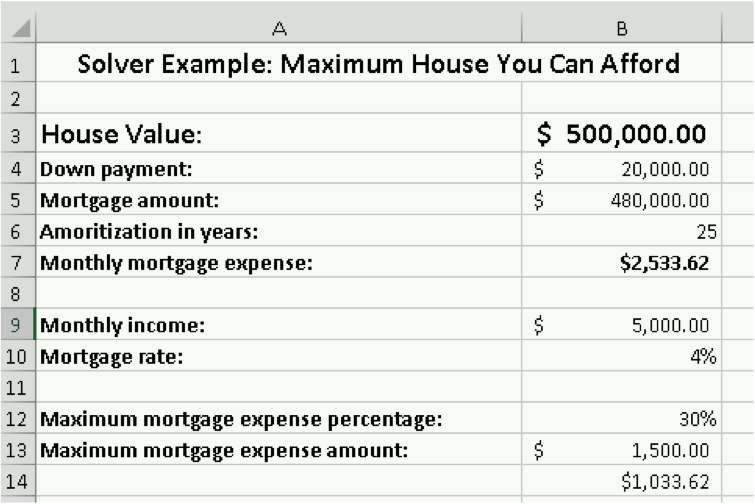
\includegraphics[height=.45\textheight,valign=t]{Linear1}|}
\begin{center}
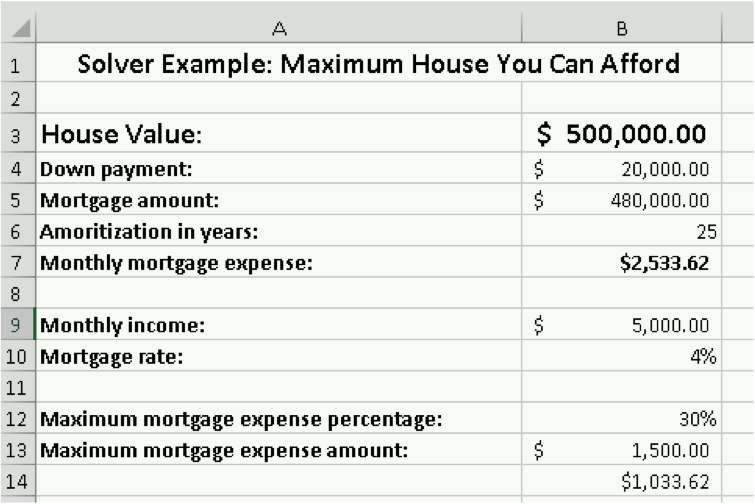
\includegraphics[height=.45\textheight,valign=t]{Linear1}
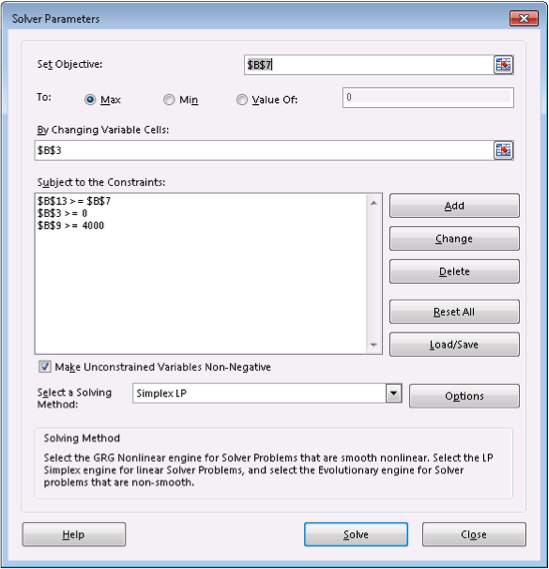
\includegraphics[width=.45\textwidth,valign=t]{Linear2}
\end{center}
\end{frame}

\begin{frame}
\begin{center}
\begin{tikzpicture}
  \node (img1) {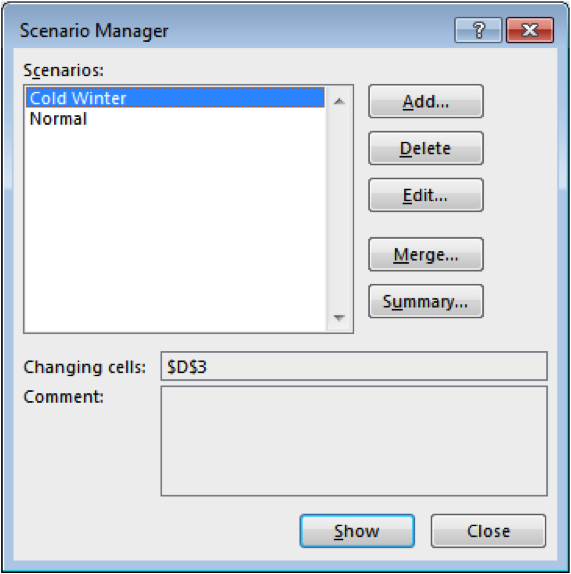
\includegraphics[height=3cm]{whatif1}};
  \pause
  \node (img2) at (img1.south east) {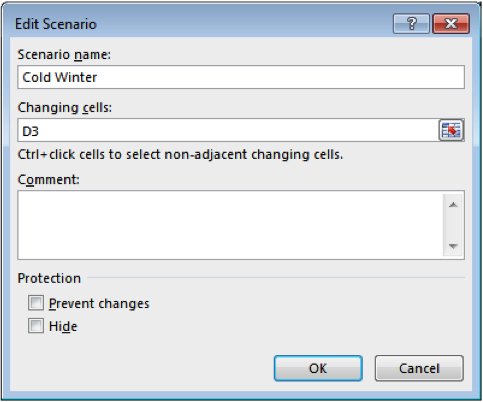
\includegraphics[height=3cm]{whatif2}};
  \pause
  \node (img3) at (img2.south west) [yshift=1cm] {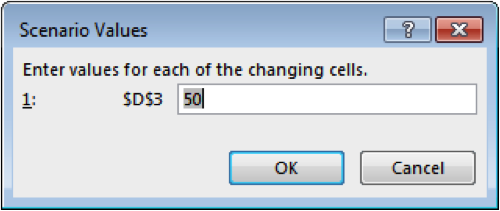
\includegraphics[height=3cm]{whatif3}};
\end{tikzpicture}
\end{center}
\end{frame}





\begin{frame}[label=current, t]
\frametitle{Outils}
\begin{block}<1->{Whatever}
  \begin{itemize}
    \item<2-> items
    \item<5-> go here
  \end{itemize}
\end{block}



\begin{onlyenv}<3-6>
  \begin{center}
    \includegraphics<3>[scale=0.4]{whatif1}
    \includegraphics<4>[scale=0.4]{whatif2}
    \includegraphics<6>[scale=0.4]{whatif3}
  \end{center}
\end{onlyenv}

\begin{onlyenv}<7->
  \begin{block}<7->{Scores}
    \begin{itemize}
      \item<8-> CRPS et MAE
      \item<9-> Diagramme de Talagrand
      \item<11-> Diagramme de fiabilit
    \end{itemize}
  \end{block}
\end{onlyenv}
\begin{center}
  \includegraphics<10>[scale=0.2]{whatif1}
  \includegraphics<10>[scale=0.2]{whatif2}
\end{center}

\end{frame}


\section{uncover}

\begin{frame}
\begin{multicols}{2}
\begin{enumerate}
    \item a
    \item b
    \item c
    \item d
    \item e
    \item f
\end{enumerate}
\end{multicols}\end{frame}

\begin{frame}
\begin{enumerate}[A]
\item<2-5> James Madison
\item<3-5> Harry Truman
\item<4-> \color<6>[rgb]{0,0.6,0}Abraham Lincoln
\item<5-5> Calvin Coolidge
\end{enumerate}
\uncover<1-5>{Hints:}\\
\uncover<2-5>{James Madison ate broccoli.}\\
\uncover<3-5>{Harry Truman drank milk.}\\
\uncover<4-5>{Abe Lincoln raised bees.}\\
\uncover<5-5>{And Cal Coolidge grew silk.}\\
\end{frame}

\begin{frame}[fragile]{Advanced Spreadsheet Addressing}
You can three different ways you can specify an absolute address
\begin{itemize}
\item By row eg. \verb|=B$1|
\item By column eg. \verb|=$B1|
\item By cell (row and column) eg. \verb|=$B$1|
\end{itemize}
  \begin{exampleblock}{}
Question: How would the formula \verb|=$A2+B$3| in cell \cell{D3} be changed when copied to \cell{E5}?  \end{exampleblock}
\only<beamer:2-|handout:0>{\cell{D3} to \cell{E5}:  $\rightarrow$ one column, $\downarrow$ two rows\\}
\begin{itemize}
\item<beamer:3-|handout:0>{\verb|$A2|:  + \st{$\rightarrow$ one column}, $\downarrow$ two rows = \verb|$A4|\\}
\item<beamer:4-|handout:0> {\verb|B$3|:  + {$\rightarrow$ one column}, + \st{$\downarrow$ two rows} = \verb|C$3|\\}
\end{itemize}
\begin{block}<beamer:5-|handout:0> 
{}Answer: The copied formula would appear as \verb|=$A4+C$3| in cell \cell{E5}
\end{block}
\end{frame}


\begin{frame}
% The beamer command \alt<*overlay specification*>{foo}{bar} will insert foo if the current slide is within the given overlay specification, and bar otherwise.
\begin{align*}
y &= \frac{(x^2+1)\sqrt{x+3}}{x-1} \\
\ln y &= \ln (x^2+1) + \frac{1}{2} \ln(x+3) - \ln(x-1) \\
\frac{1}{y} \frac{dy}{dx}
      &= \frac{2x}{x^2+1} + \frac{1}{2(x+3)} - \frac{1}{x-1}
\end{align*}
So
\[
\begin{split}
\frac{dy}{dx} &= \left(\frac{2x}{x^2+1} + \frac{1}{2(x+3)} - \frac{1}{x-1}
\right)
\alt<2>{\frac{(x^2+1)\sqrt{x+3}}{x-1}}{y}
\end{split}
\]
\end{frame}

\section{question}



%%%%%%%%%%%%%%%%%%%%%%%%%

% question:

\begin{frame}[fragile]\ft{}
  \begin{example}
PlaceQuestionHere
\begin{enumerate}
\item {{Option1}}
\item {{Option2}}
\item {{Option3}}
\item {{Option4}} 
\end{enumerate}
\begin{multicols}{5}
\begin{enumerate}[A)]
\item 0 
\item 1
\item 2
\item 3
\item 4
\end{enumerate}
\end{multicols}
  \end{example} 
\end{frame}


% answer:

\begin{frame}<handout:0>[fragile]\ft{}
  \begin{block}{Answer:}
PlaceQuestionHere
\begin{enumerate}
\item {\color<1->{sgreen}	{Option1}}
\item {\color<2->{red}	{Option2}}
\item {\color<3->{sgreen}	{Option3}}
\item {\color<4->{red}	{Option4}} 
\end{enumerate}
\begin{multicols}{5}
\begin{enumerate}[A)]
\item 0 
\item 1
\item 2
\item \tans{5}{3} 
\item 4
\end{enumerate}
\end{multicols}
  \end{block} 
\end{frame}


%%%%%%%%%%%%%%%%%%%%%%%%%








\begin{frame}{Aggregate Functions Question}
  \begin{block}{Answer:}
Assume the cells in the range {\tt A1:C4} each contain a number that is equal to their row number (e.g. \blue{B3} contains {\tt 3}). How many of the following statements are TRUE?
\begin{enumerate}
\item {\color<2->{sgreen}{The number of cells in the range is 12.}}
\item {\color<3->{red}{The value of {\tt SUM(A1:C4)} is 20}. }
\item {\color<4->{sgreen}{The value of {\tt COUNTIF(A1:B4,">2")} is 4}.}
\item {\color<5->{red}{\tt AVERAGE(A1:C4) > MAX(C2:C3)}} 
\end{enumerate}
\begin{multicols}{5}
\begin{enumerate}[A)]
\item 0 
\item 1
\item 2
\item \textbf<6>{\textit<6>{{\color<6>{iyellow}{3}}}}
\item 4
\end{enumerate}
\end{multicols}
  \end{block} 
\end{frame}


\begin{frame}
  \begin{exampleblock}{Question:}
Is the answer yes or no? {\color<beamer:2|handout:0>{sgreen}{yes}}   B) no
  \end{exampleblock} 
  \pause\pause
This answer (which appears in the form of coloured text) will only appear on beamer slides but NOT the handout. Put a double pause in order to get a slide with JUST the colour change
\end{frame}





\begin{frame}
  {Equations}

  Equations are easy
  \begin{itemize}
  \item Just copy/paste equations\pause
  \item From the paper!
    \begin{equation*}
      \textbf{p}^* = \underset{\textbf{p}}{\arg\!\min}~\sum_{\textbf{x}}\left[ I(\textbf{W}(\textbf{x};\textbf{p})) - T(\textbf{x}) \right]^2
    \end{equation*}
  \end{itemize}
\end{frame}





\begin{frame}
  {A Movie}

  \begin{block}{Some block}
    \begin{itemize}
    \item Movies only seem to work in Adobe Reader
    \item Movie file is not embedded, it must be on the computer
    \end{itemize}
  \end{block}

  \begin{exampleblock}{Some more block}
    Movies only seem to work in Adobe Reader\par
    Movie file is not embedded, it must be on the computer
  \end{exampleblock}

  \begin{alertblock}{}
    Some text in here.
    \begin{itemize}
    \item Movies only seem to work in Adobe Reader
    \item Movie file is not embedded, it must be on the computer
    \end{itemize}
  \end{alertblock}
\end{frame}

\begin{frame}<handout:0>
This frame won't be included in the handout mode
\end{frame}


\begin{frame}[fragile]
We need "fragile" frame to use verbatim \verb|see()#|
This is how we do lettered lists:
\begin{enumerate}[A)]
\item  0		
\item 1		
\item 2		
\item \emph{\yellow 3}		
\item 4
\end{enumerate}

 \begin{itemize} \setlength{\itemsep}{0pt}
\item no space 
\item between bullets
\end{itemize}


 \begin{itemize} \setlength{\itemsep}{5pt}
\item be sure
\item to set back
\item to 5pt sep
\end{itemize}


\end{frame}






\begin{frame}
  {Credits}

  \begin{itemize}
  \item Brought to you by Cédric Mauclair
  \item Please let me know about improvements!
  \item inspiration: \url{http://www.shawnlankton.com}... (in code)
  \end{itemize}
\end{frame}


\begin{frame}
  {Questions}

  \nocite{lorem,ipsum}
  \bibliographystyle{plain}
  \bibliography{../demo}

\end{frame}

\end{document}

